%! Author = Kiddo_Tsukuyomi
%! Date = 

% Preamble
\documentclass[UTF8]{ctexart}

% Packages
\usepackage{geometry}
\usepackage{listings}
\usepackage{xcolor}
\usepackage{graphicx}
\usepackage{amsmath}
\usepackage{subcaption}

% Settings
\lstset{
    backgroundcolor=\color{gray!5}, % Code block background color
    basicstyle=\ttfamily\small, % Font style: monospaced, small size
    columns=fullflexible, % Allow line wrapping, no restrictions on column number
    keepspaces=true, % Preserve spaces
    language=[LaTeX]TeX, % Code language is LaTeX
    breaklines=true, % Allow automatic line breaking
    breakatwhitespace=true, % Break at whitespace only
    postbreak=\mbox{\textcolor{red}{$\hookrightarrow$}\space}, % Mark break position with red arrow
    commentstyle=\color{gray}\itshape, % Comment style: gray italic
    stringstyle=\color{orange}, % String style: orange
    keywordstyle=\color{blue}, % Keyword style: blue
    showstringspaces=false, % Do not show spaces within strings
    numbers=left, % Display line numbers on the left
    numberstyle=\scriptsize, % Line number font size: footnote size
    numbersep=8pt, % Distance between line numbers and code: 8pt
    frame=single, % Add single line border
    frameround=tttt, % Rounded corners for the frame
    rulecolor=\color{black}, % Frame color: black
    extendedchars=true, % Allow the use of extended character sets
    inputencoding=utf8, % Input encoding: UTF-8
    literate={~} {$\sim$}{1}, % Handle tilde symbol display
    escapeinside=``, % Use backticks as an escape region, to avoid garbled characters when using Chinese text
    xleftmargin=2em, % Left margin of the code block
    xrightmargin=2em, % Right margin of the code block
    aboveskip=1em, % Space above the code block
    framexleftmargin=2em, % Left margin of the frame
}

% Document
\begin{document}
	\title{\textbf{HW10}}
	\author{白博臣、何骐多、夏营}
	\date{}
	\maketitle

    \begin{figure}[h]
        \centering
        \begin{minipage}{0.32\textwidth}
            \centering
            \includegraphics[width=\linewidth]{bbc}
            \caption{白博臣}
            \label{fig:img1}
        \end{minipage}\hfill
        \begin{minipage}{0.305\textwidth}
            \centering
            \includegraphics[width=\linewidth]{hqd}
            \caption{何骐多}
            \label{fig:img2}
        \end{minipage}\hfill
        \begin{minipage}{0.32\textwidth}
            \centering
            \includegraphics[width=\linewidth]{xy}
            \caption{夏营}
            \label{fig:img3}
        \end{minipage}
    \end{figure}

    \section{Problem1}\label{sec:section1}
    \subsection{a}\label{subsec:1.1}
    直接使用 Romberg 积分,第一个积分被积函数 \(\sqrt{1 - x^2}\),上下限 -1, 1。用这个作为参数,调用 \texttt{IntegrationPrecise()}。

    第二个积分被积函数 \(\sin^2{x}\),上下限 0,\(\pi\)。用这个作为参数,调用 \texttt{IntegrationPrecise()}。

    \subsection{b}\label{subsec:1.2}
    在对第一个积分进行数值积分时,\(\theta = \theta_0\)时,分母会变为0,为避免出现 \texttt{Infinity},将分母添加一个小量,避免除以0,再进行积分。

    \subsection{c}\label{subsec:1.3}
    对原式进行如下变形
    \begin{equation*}
        \begin{align*}
            I & = \int_{0}^{\infty} \frac{dx}{(1 + x) \sqrt{x}} \\
              & = \int_{0}^{1} \frac{dx}{(1 + x) \sqrt{x}} + \int_{1}^{\infty} \frac{dx}{(1 + x) \sqrt{x}} \\
              & = \int_{0}^{1} \frac{dx}{(1 + x) \sqrt{x}} + \int_{1}^{0} \frac{d\left( \frac{1}{x})}{\left(1 + \frac{1}{x}\right) \sqrt{\frac{1}{x}}} \\
              & = 2 \int_{0}^{1} \frac{dx}{(1 + x) \sqrt{x}} \\
        \end{align*}
    \end{equation*}

    使用 \texttt{Java} 代码实现,见附件 \texttt{IntegrationDiscreteCal1.java},运行结果如下
    \begin{figure}[h]
        \centering
        \includegraphics[height=0.08 \textheight]{fig1_1}
        \caption{a 题结果}\label{fig:figure1.1}
    \end{figure}
    \begin{figure}[h]
        \centering
        \includegraphics[height=0.4 \textheight]{fig1_2}
        \caption{b 题结果}\label{fig:figure1.2}
    \end{figure}
    \begin{figure}[h]
        \centering
        \includegraphics[height=0.04 \textheight]{fig1_3}
        \caption{c 题结果}\label{fig:figure1.3}
    \end{figure}

    \newpage
    \section{Problem2}\label{sec:section2}
    对于此问题,所求积分为无穷积分,为使用数值积分的方法对其进行处理,这里需要采取变量代换的方式。为方便代换,不妨考虑将高斯积分置于极坐标系下进行变换,即对积分式:
    \begin{equation*}
        I^2 = \int_{-\infty}^{\infty} e^{-x^2} d x \int_{-\infty}^{\infty}
    \end{equation*}
    进行变换。

    有极坐标变换:
    \begin{equation*}
        r^2 = x^2 + y^2, \quad dx dy = r dr d \theta
    \end{equation*}

    进而有:
    \begin{equation*}
        I^2 = \int_{0}^{2 \pi} d \theta \int_{0}^{\infty} r e^{-r^2} dr
    \end{equation*}

    从而可以将 \(I^2\) 分解成两个定积分的乘积:
    \begin{equation*}
        I^2 = I_1 \cdots I_2, \quad I_1 = \int_{0}^{2 \pi} d \theta, \quad I_2 = \int_{0}^{\infty} r r^{-r^2} dr
    \end{equation*}

    可以发现对于 \(I_2\) ,其仍是一个无穷积分,因此需要进行进一步的变量代换,令:
    \begin{equation*}
        t = e^{-r^2}, \quad dt = de^{-r^2} = -2 r e^{-r^2} dr
    \end{equation*}

    得到:
    \begin{equation*}
        I_2 = \int_{0}^{1} \frac{1}{2} dt
    \end{equation*}

    由此 \(I_1\) 与 \(I_2\) 均化作了可以使用数值积分计算的形式。

    这里使用上次作业所实现的 Simpson’s Rule ,选取 49 个点进行计算。

    计算结果如下:
    \begin{figure}[h]
        \centering
        \includegraphics[height=0.04 \textheight]{Figuer2}
        \caption{运行结果}\label{fig:figure2}
    \end{figure}

    \section{Problem3}\label{sec:section3}

    使用 \texttt{Java} 代码实现,见附件 \texttt{IntegrationDiscreteCal2.java},运行结果如下
    \begin{figure}[h]
        \centering
        \includegraphics[height=0.32 \textheight]{fig3}
        \caption{运行结果}\label{fig:figure3}
    \end{figure}

    \newpage
    \section{Problem4}\label{sec:section4}
    \subsection{a}\label{subsec:section4.1}
    由题干可知,\(q(u)\) 为光的传输函数,其对应的是光在离中心轴的距离为 \(u\) 的地方的透过率,而唯有当光正好通过光栅狭缝时,\(q(u)\) 有最大值。因此光栅狭缝之间的间隔,即为 \(q(u)\) 最大值之间的间隔。
    \begin{equation*}
        q(u) = \sin^2 \alpha u
    \end{equation*}

    所以有间隔:
    \begin{equation*}
        T = \frac{\pi}{\alpha}
    \end{equation*}

    进而有:
    \begin{equation*}
        d = \frac{\pi}{\alpha}
    \end{equation*}

    \subsection{b}\label{subsec:section4.2}
    \texttt{Python} 代码如下:
    \begin{lstlisting}[language=Python, breaklines = true,label={lst:lstlisting1}]
import numpy as np
def q(u):
d=0.00002
alpha=np.pi/d
return np.sin(alpha*u)**2
    \end{lstlisting}

    \subsection{c}\label{subsec:section4.3}
    对于此题,先将题干中的所有数据列出如下:

    光栅狭缝间隙:\(d = 0.00002 m\)

    光栅总长度:\(w = d \times 10 = 0.0002 m\)

    屏幕宽度:\(l = 0.1 m\)

    焦距:\(f = 1 m\)

    入射光波长:\(\lambda = 0.0000005 m\)

    利用上一问中的 \(q(u)\) 的代码,再依次将数据代入被积函数中,使用 Simpson’s Rule 进行积分即可得出结果。

    其中,由光栅方程:
    \begin{equation*}
        d\sin \theta = k \lambda
    \end{equation*}
    其中k为主级大的阶数,可以给出一阶主级大所在位置为:
    \begin{equation*}
        x = \pm 0.025 m
    \end{equation*}
    为此,可以以此为判断根据来选择Simpson’s Rule所用的样本点数。在进行了多次试探以后,我们发现当样本点数为49个时,即可得到十分相近的光强分布图,所以我们可以认为此时的积分结果是准确的。
    仿真结果如下:
    \begin{figure}[h]
        \centering
        \includegraphics[height=0.42 \textheight]{problem4_c}
        \caption{仿真结果}\label{fig:figure4.3}
    \end{figure}

    \subsection{d}\label{subsec:section4.4}
    为实现可视化,我们使用灰度图的方式来模拟屏幕上条纹的分布,其中用到了 \texttt{python matplotlib.pyplot} 库中的 \texttt{imshow} 函数。

    实现结果如下
    \begin{figure}[h]
        \centering
        \includegraphics[height=0.42 \textheight]{problem4_d}
        \caption{仿真结果}\label{fig:figure4.4}
    \end{figure}

    \newpage
    \subsection{e}\label{subsec:section4.5}
    \subsubsection{i}\label{subsubsec:section4.5.1}
    对前面的仿真代码中修改 \(q(u)\) 函数即可,即此时有:
    \begin{equation*}
        q(u) = \sin^2 \alpha u \sin^2 \beta u
    \end{equation*}
    其中,\(\beta = \frac{\alpha}{2}\)。

    实现结果如下;
    \begin{figure}[h]
        \centering
        \begin{minipage}[b]{0.4\textwidth}
            \centering
            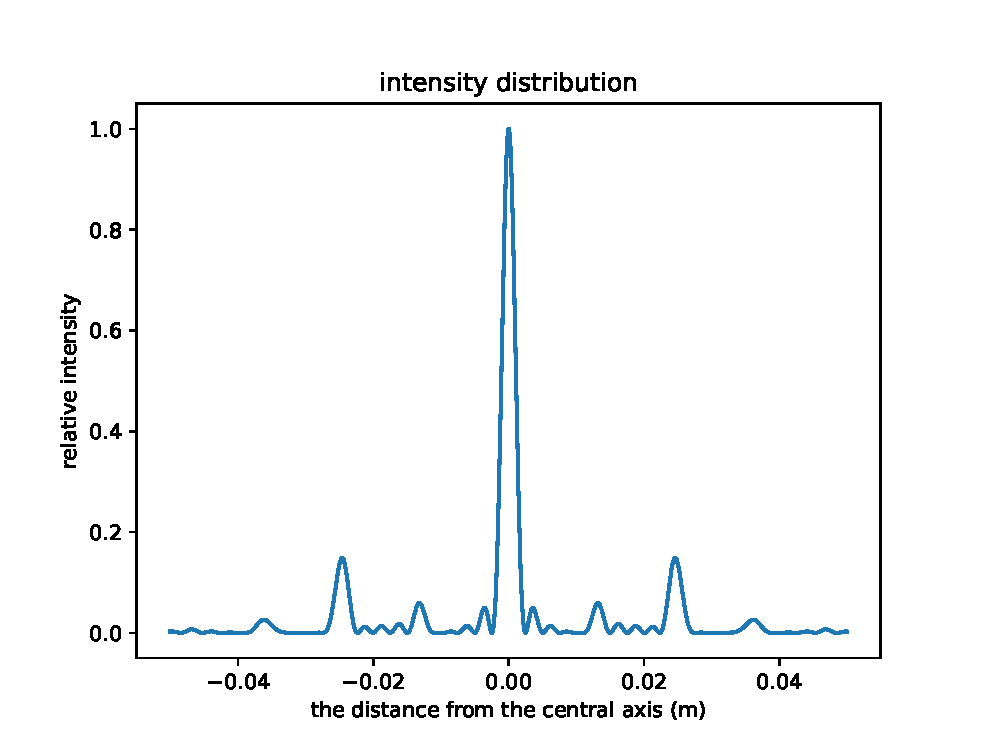
\includegraphics[height=0.28 \textheight]{problem4_e(i)_1}
            \label{fig:figure4.5.1.1}
        \end{minipage}
        \hfill
        \begin{minipage}[t]{0.4\textwidth}
            \centering
            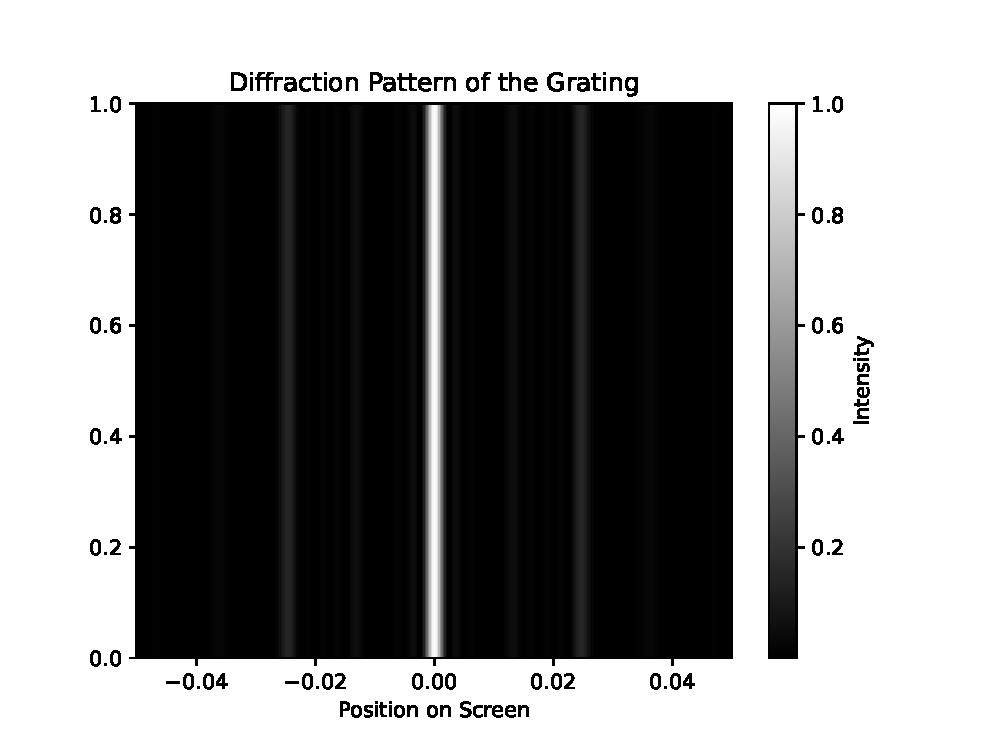
\includegraphics[height=0.32 \textheight]{problem4_e(i)_2}
            \label{fig:figure4.5.1.2}
        \end{minipage}
        \caption{仿真结果}
    \end{figure}

    \newpage
    \subsubsection{ii}\label{subsubsec:section4.5.2}
    此时的 \(q(u)\) 为分段函数,即:
    \begin{equation*}
        q(u) = \left\{ \begin{align*}
                           & 1, \quad u \leq -0.000025 \, or \, u \geq 0.000035 \\
                           & 0, \quad others \\
        \end{} \right\}
    \end{equation*}

    同时,光栅的总宽度也发生了变化,即:
    \begin{equation*}
        w = 0.00009 m
    \end{equation*}

    实现结果如下:
    \begin{figure}[h]
        \centering
        \begin{minipage}[b]{0.4\textwidth}
            \centering
            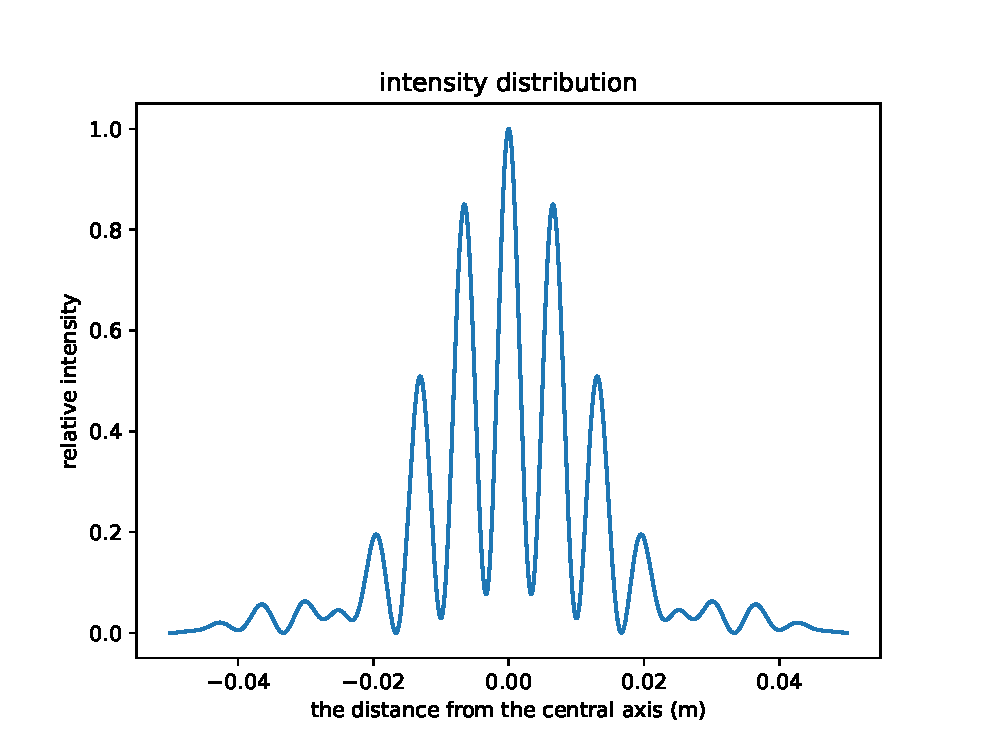
\includegraphics[height=0.28 \textheight]{problem4_e(ii)_1}
            \label{fig:figure4.5.2.1}
        \end{minipage}
        \hfill
        \begin{minipage}[t]{0.4\textwidth}
            \centering
            \includegraphics[height=0.32\textheight]{problem4_e(ii)_2}
            \label{fig:figure4.5.2.2}
        \end{minipage}
        \caption{仿真结果}
    \end{figure}

    \newpage

    \section{Problem 5}
    \subsection{问题回顾}
    利用传统的积分方法计算多维球的体积,并将计算结果作图分析。
    \subsection{问题解答}
    我们参考了以下n维球体积计算公式:

    \[V_n=\frac{\pi^{\frac{n}{2}R^n}}{\Gamma(\frac{n}{2}+1)}=C_nR^n\]
    \[C_n=\frac{\pi^k}{k!} (For Even n=2k)\]
    \[C_n=C_{2k+1}=\frac{2^{2k+1}k!\pi^k}{(2k+1)!} (For odd n=2k+1)\]

    \subsubsection{坐标与数组}
    $x$维坐标数组,$x\left[k\right]$表示$k$维坐标,A为一维的权重数组,对应计算积分时取得权重值。
    \subsubsection{宏定义和全局变量}

    使用 \textbf{\#define} 定义了圆周率 $\pi$。\textbf{n} 表示每个维度中用于积分的点数。\textbf{N} 是多维空间的维度数。\textbf{sum} 是用于累积积分结果的变量。\textbf{step} 表示每个维度的步长。\textbf{start} 和 \textbf{end} 是用来测量程序执行时间的变量。

    \subsubsection{阶乘和双阶乘函数}

    \textbf{factorial} 函数计算给定正整数$ m $的阶乘。\textbf{double\_factorial} 函数计算给定正整数 $m $的双阶乘,这是$ m!! $的定义,只计算 $m, m-2, m-4, \dots$ 直到1。

    \subsubsection{计算多维球体积的真实值函数}
    \textbf{n\_dimensional} 函数根据维度数的奇偶性选择不同的数学公式来计算多维球体积的精确值。不同的维度数需要不同的数学公式来计算其体积。

    \subsubsection{函数 fx}
    \textbf{fx} 函数根据传入的点 $x $判断该点是否位于单位球内部。如果在单位球内部,返回1;否则返回0。这个函数用于积分计算过程中的判断条件。

    \subsubsection{递归计算积分值的函数 Circulation}

    \textbf{Circulation} 函数通过递归计算多维空间中球体积的近似值。它接受当前维度的索引$ k$,当前积分点的数组 $X$,当前权重数组 $A$,和当前的步长 $a$。递归地计算每个维度的积分点,累加权重乘积来逼近球体积的积分值。

    其核心为递归法,根据积分公式有:
    \[\overset{(N)}{\int}f(x_1,x_2,\dots,x_N)dx_1 dx_2 \dots dx_N=\sum_{i}A_i\overset{(N-1)}{\int}f(x1,\dots,x_{N-1},x_{N_i})dx_1dx_2\dots dx_{N-1}\]

    根据这一关系,可以得到Circulation(k,x,A,a)函数递归关系如下:
    \[Circulation(k, x, A, a) = \sum_{i}*Circulation(k-1, x, A, a)(x_k=x_{k_{i}})\]
    \[=\sum_{i}Circulation(k-1, x, A, A_i * a)(x_k=x_{k_{i}})\]

    在$k<0$时$sum=sum+a*fx$,最终可以计算出结果sum.
    \subsubsection{函数 findn}
    \textbf{findn} 函数根据给定的维度数 N,选择合适的点数 n,即每个维度的分段数。这个选择影响了积分的精度和计算效率。

    利用gnuplot作出计算体积图以及误差图:

    \begin{figure}[htbp]
        \centering
        \includegraphics[height=8cm]{V.png}
        \caption{计算体积与计算维数关系图}
    \end{figure}

    \begin{figure}[htbp]
        \centering
        \includegraphics[height=8cm]{E.png}
        \caption{计算误差与计算维数关系图}
    \end{figure}

    可以看出,误差基本都在5\%以内,可见计算结果还是比较准确。为加速计算,在高维减少了取点数,控制误差在5\%以内。高维虽然取点较少,但实际上参与计算的积分的坐标点较多,也就时参与计算的体积元较多,所以对结果影响不是非常大,最后在用积分公式计算时就表现出较小的误差。

\end{document}
